% Budget: ~1.5 columns  |  13 pts.  Slides p.10-11.
% Sources: results/README.md (I2), model/report/P3_model_choice_and_results.md,
%          model/results/tables/model_choice/model_choice_evidence.csv (P3).
\section{Method}
\label{sec:method}

\begin{figure*}[t]
\centering
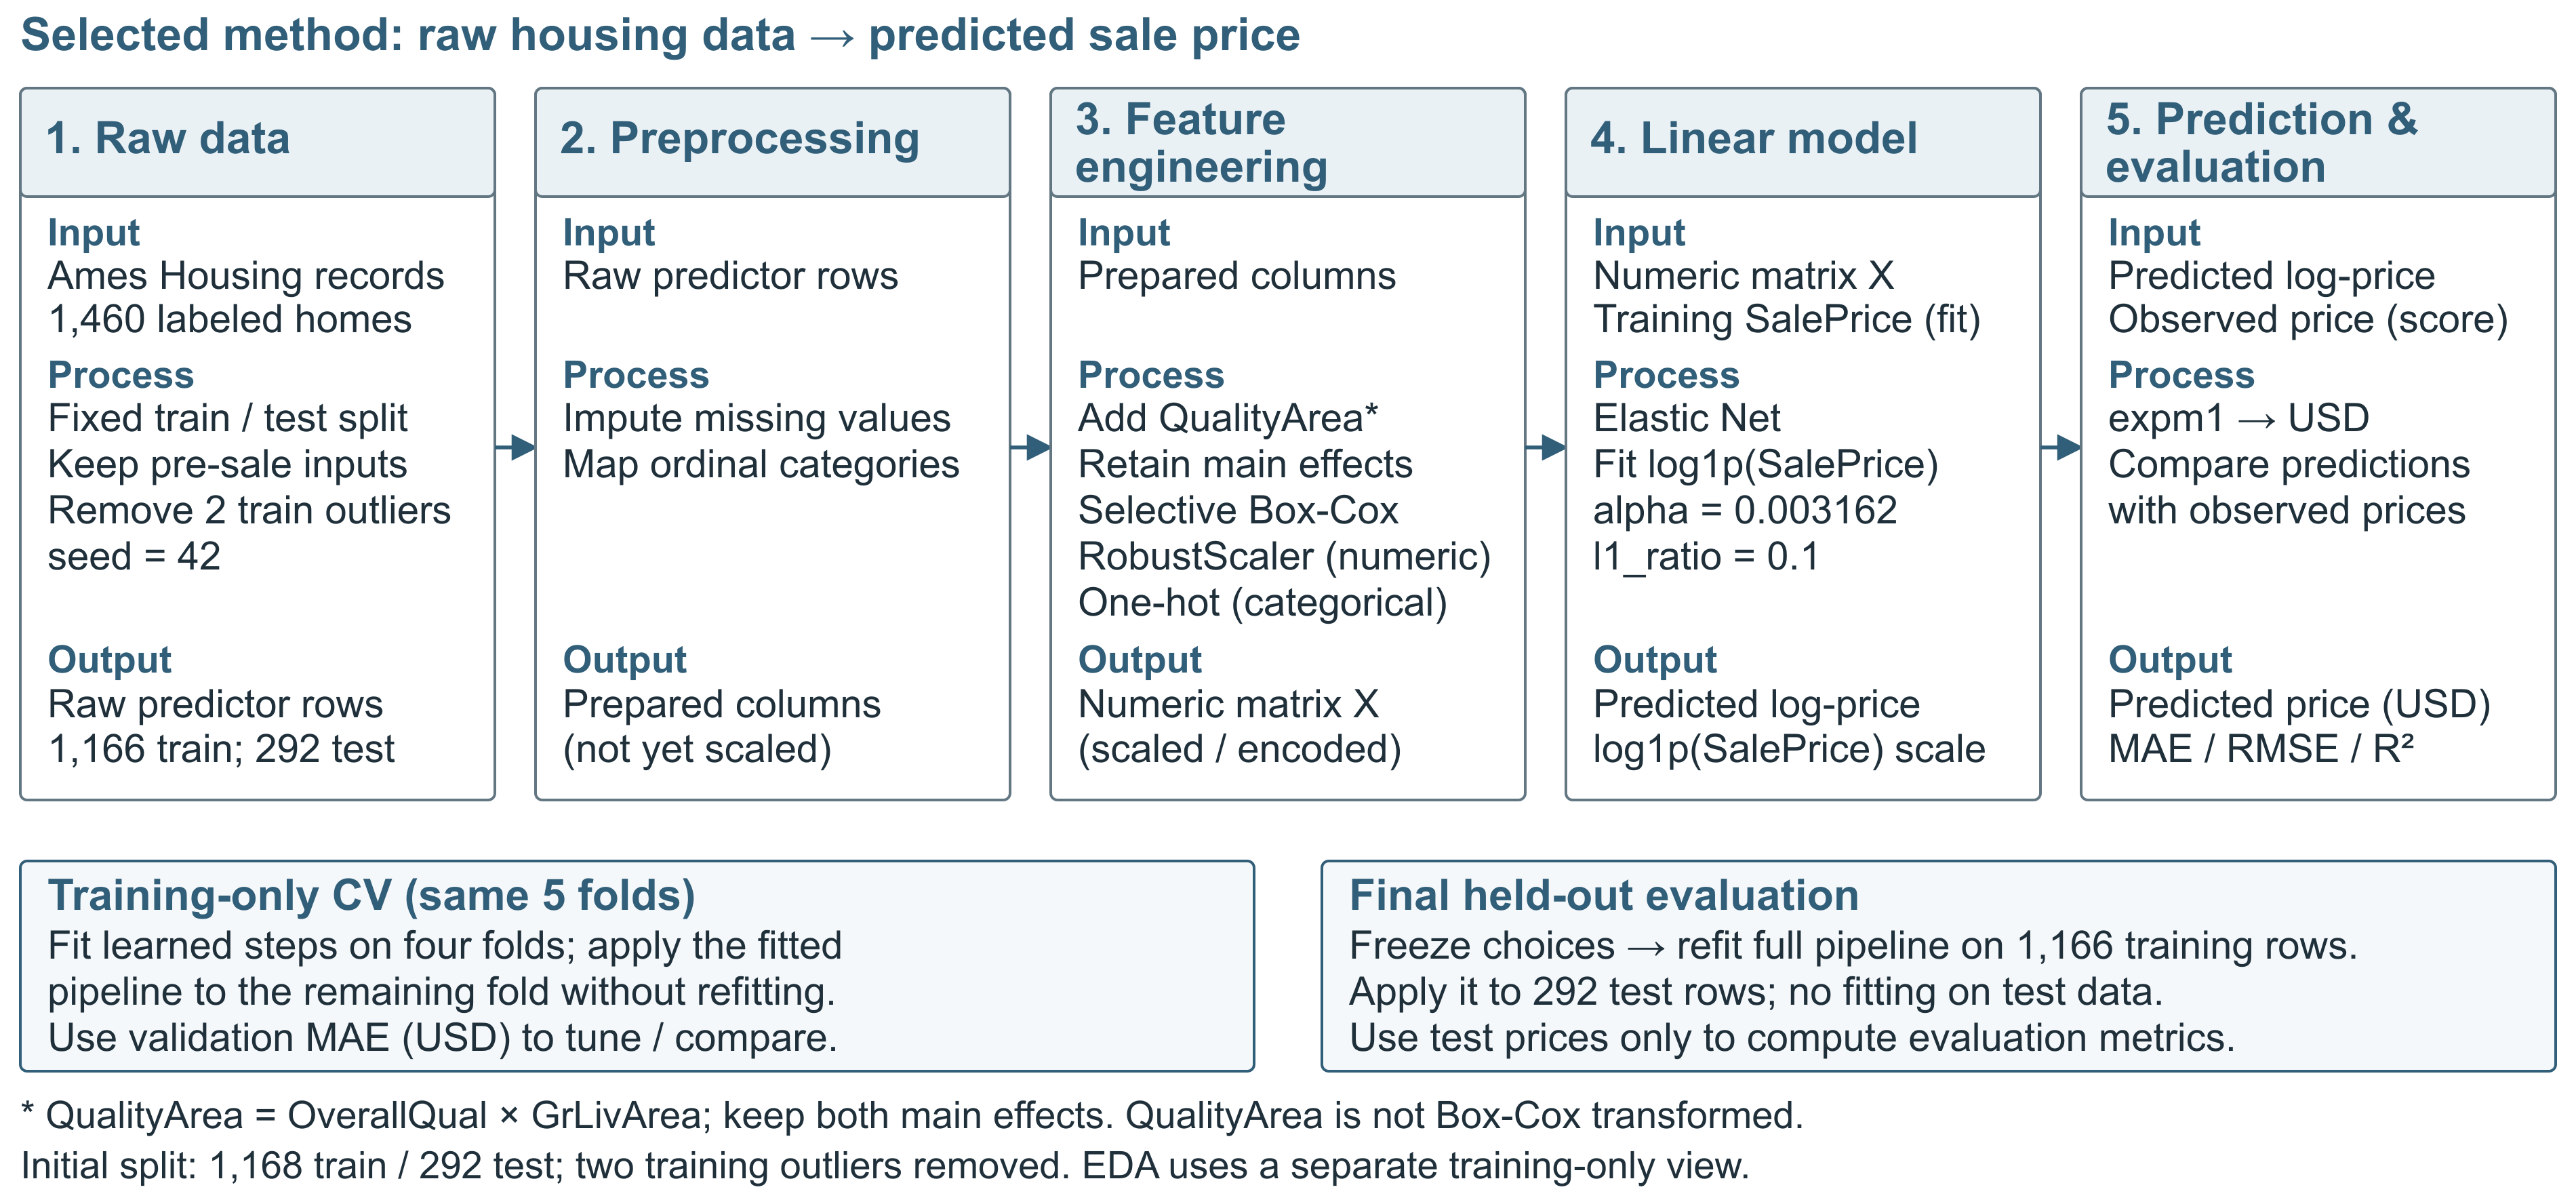
\includegraphics[width=0.95\textwidth]{figures/pipeline.png}
\caption{Five-stage pipeline from raw records to predicted sale prices, with each stage's input, processing and output. Learned steps are fitted within each training fold only; after all choices are frozen, the pipeline is refitted on 1,166 training rows and applied once to 292 test rows.}
\label{fig:pipeline}
\end{figure*}

\subsection{Pipeline and Feature Engineering}
Figure~\ref{fig:pipeline} shows the full pipeline. We designed one feature group per hypothesis.
\textbf{Interaction (H1):} QualityArea lets a linear model give each square foot a value that rises with quality; both main effects are kept.
\textbf{Transform (H2):} LogLotArea captures diminishing returns to land.
\textbf{Aggregate (H3):} TotalSF summarizes floor area in one column.
Only QualityArea is used in the final model (\S\ref{sec:results}).

\subsection{Model Choice and Hyperparameter Tuning}
The data have strongly correlated attribute groups and over 200 encoded predictors, many of them weak.
OLS is unstable here: its coefficients are not unique under rank deficiency, and it is our weakest linear model (CV MAE 14{,}958~USD).
Ridge \citep{hoerl1970ridge} handles collinearity but keeps all 209.8 predictors on average.
Lasso \citep{tibshirani1996lasso} removes weak predictors, but within a correlated group it tends to keep one member arbitrarily.
We therefore use Elastic Net \citep{zou2005elastic}, which combines both penalties and keeps 113.4 non-zero coefficients on average.
Its standardized coefficients are also stable across folds (mean pairwise cosine 0.960 vs.\ 0.954 for Lasso).
Its CV MAE ties with Lasso's (13{,}366 vs.\ 13{,}361~USD, a gap far below the fold SD of about 800~USD), so the choice rests on data structure rather than on the score.

We tune by grid search on the five training folds, minimizing MAE in USD.
The ranges are $\alpha \in [10^{-5}, 1]$ (11 log-spaced values) for Lasso and Elastic Net, with L1 ratio $\in \{0.1, 0.5, 0.9\}$ for the latter, and $\alpha \in [10^{-3}, 10^4]$ (15 values) for Ridge.
The selected Elastic Net uses $\alpha = 0.00316$ and an L1 ratio of 0.1, i.e., mostly L2 shrinkage with modest sparsity.
